\documentclass[11pt]{article}
\usepackage[T1]{fontenc}
\usepackage[margin=1in]{geometry}
\usepackage{amsmath,amssymb,amsthm,booktabs,microtype,tikz}
\usetikzlibrary{arrows.meta,positioning,calc}
\usepackage[hidelinks]{hyperref}
\newtheorem{theorem}{Theorem}[section]
\newtheorem{proposition}[theorem]{Proposition}
\newtheorem{lemma}[theorem]{Lemma}
\newtheorem{corollary}[theorem]{Corollary}
\theoremstyle{definition}
\newtheorem{definition}[theorem]{Definition}
\newtheorem{example}[theorem]{Example}
\newtheorem{remark}[theorem]{Remark}
\newcommand{\Aut}{\operatorname{Aut}}
\newcommand{\Bij}{\operatorname{Bij}}
\newcommand{\Sym}{\operatorname{Sym}}
\newcommand{\Id}{\mathcal J}
\newcommand{\Lin}{\mathcal L}
\newcommand{\Z}{\mathbb Z}
\newcommand{\Q}{\mathbb Q}
\newcommand{\E}{\mathbb E}
\newcommand{\CAT}{\operatorname{CAT}}
\numberwithin{equation}{section}
\title{Causal Histories, Observable States, and Cubical Geometry}
\author{Alexander Kolpakov\\[0.5ex]
\small Center for Science, Technology, Engineering, and Mathematics\\
\small University of Austin, Austin, Texas, United States\\
\small \texttt{akolpakov@uaustin.org}\\[0.75ex]
\small The Wolfram Institute for Computational Foundations of Science\\
\small \texttt{akolpakov@wolframinstitute.org}}
\date{Research note, 20 October 2026}
\begin{document}
\maketitle
\begin{abstract}
Finite hypergraphs and token-replacement histories have explicit
presentations by restrictions of permutation torsors. Their symmetry
quotients retain the usual inverse-automorphism weights; forgetting
the order of events introduces an additional linear-extension factor.
For a fixed occurrence history, prefixes form the familiar CAT(0)
cube complex of ideals of a causal poset. We give a direct criterion
for an observation of those prefixes to inherit their median operation:
its fibres must be obtained by forgetting a fixed subset of events.
For additive token observations this becomes an exact condition on
the integer effect matrix, with a finite witness whenever it fails.
Finally, terminating confluent one-token systems can have state
complexes with fundamental group of any positive finite free rank, although
their history unfoldings are trees. The results distinguish geometry
of occurrences from geometry of observable states.
\end{abstract}

\section{Introduction}
An occurrence history records which event produced each token, which
event consumed it, and which events depended on earlier ones.
An observable state may retain only the tokens currently present.
These are different objects. In particular, identifying occurrences
with the same observable state need not preserve their geometry.

The geometry of event structures and state complexes is established
theory. Nielsen--Plotkin--Winskel \cite{NPW} relate Petri nets,
event structures and domains. Ghrist--Peterson \cite{GP} study cubical
state complexes for reconfiguration systems. Ardila--Owen--Sullivant
\cite[Section 2]{AOS} give a poset description of CAT(0) cube complexes.
Chalopin--Chepoi \cite[Sections 3 and 8]{CC} relate 1-safe Petri nets
to special cube complexes and describe their unfoldings using
universal covers. The prefix geometry used below is the finite,
conflict-free case of this theory.

Our setting is finite and explicit. A history consists of a fixed
inventory of token-replacement occurrences, with no absence tests or
other global application conditions. Two preserved blocks inside one
permutation torsor describe birth-to-consumption wiring and schedules.
Forgetting schedules produces a linear-extension weight, which must
be distinguished from the graph automorphism weight.

The main question concerns an observation
$\sigma:\Id(P)\to S$ of the ideals of a finite causal poset $P$.
The median of three ideals is their coordinatewise majority.
We prove that this operation is well defined on observable states
exactly when equality of observations means equality on a fixed
set of event coordinates. We then specialize the criterion to
integer token-effect matrices and give explicit witnesses to failure.
This is the finite ideal-coordinate form of established median
quotient theory; the proof here uses only convexity and parallel
event edges. See Bowditch \cite[Sections 3, 7--9]{Bowditch} for the
general median-algebra and wall framework.

A separate construction shows the limits of confluence. For any
$k\ge2$ and $L\ge3$, a graded, terminating, confluent one-token
system has a state complex with fundamental group $F_{k-1}$ and
girth $2L$. Every individual history is an interval, and the full
history unfolding is a tree. Thus confluence alone does not make
state identification preserve CAT(0) geometry.

The contribution is the explicit torsor presentation and schedule
weight, a finite proof of the observation criterion, and its
token-matrix consequences and repair bounds. The proofs use event
coordinates and the standard cubical link criterion.

\section{Permutation torsors and incidence structures}

\subsection{A torsor over the integers}
For finite sets $A,B$ of size $D$, put
$T(A,B)=\Bij(A,B)$.
The actions of $\Sym(A)$ by precomposition and $\Sym(B)$ by
postcomposition commute and are both free and transitive.
Thus $T(A,B)$ is a bitorsor; an identification with $S_D$ requires
choosing one bijection.

There is a useful integral presentation. Introduce coordinates
$p_{ab}$, $a\in A$, $b\in B$, and impose
\begin{align}\label{eq:permutation}
 p_{ab}^2&=p_{ab},&
 p_{ab}p_{ac}&=0\quad(b\ne c),&
 p_{ab}p_{cb}&=0\quad(a\ne c),\\
 \sum_b p_{ab}&=1,& \sum_a p_{ab}&=1.\nonumber
\end{align}

\begin{proposition}\label{prop:ring}
The resulting coordinate ring is $\prod_{\tau\in T(A,B)}\Z$.
It represents the constant permutation torsor over $\Z$.
\end{proposition}
\begin{proof}
For each bijection $\tau$, set $e_\tau=\prod_a p_{a,\tau(a)}$.
These are pairwise orthogonal idempotents. Expanding the product of
the row sums gives $\sum_\tau e_\tau=1$: every noninjective choice
vanishes by column orthogonality. Moreover,
$p_{ab}=\sum_{\tau(a)=b}e_\tau$.
Hence the ring is generated by these components. Evaluation at each
permutation identifies its component with $\Z$, proving the claim.
Composition of bijections gives the asserted torsor actions.
\end{proof}

A forbidden finite pattern of wires $Q\subseteq A\times B$ is
excluded by $\prod_{(a,b)\in Q}p_{ab}=0$.
Such equations cut out unions of components of the torsor.
The restricted set generally has no transitive group action.
Over every field the same equations select the same finite
configurations. A coefficient-field change alone therefore adds
no metric or approximation theorem.

Orthogonality in \eqref{eq:permutation} is needed in positive
characteristic. Over $\mathbb F_2$, the $4\times4$ matrix with
zero diagonal and all other entries one is invertible and has
row and column sums one, but is not a permutation matrix.

\subsection{Graphs and their symmetry factors}
Fix vertex degrees $d_v$ and hyperedge arities $k_e$ with common sum
$D$. Partition $A=\coprod_vA_v$ and $B=\coprod_eB_e$ into blocks
of those sizes. A bijection connects an incidence at $v$ to a port
of $e$. Repeated incidences are allowed. Ordered hyperedges retain
their port order; unordered ones forget it.

Let $H_V$ consist of permutations inside the vertex blocks and
permutations of blocks of equal degree. Define $H_E$ similarly.
For coloured structures, restrict these groups to preserve colours.

\begin{proposition}\label{prop:incidence}
The action groupoid of $H_V\times H_E$ on $T(A,B)$ is equivalent
to the groupoid of incidence hypergraphs with the specified profiles.
For any invariant restriction $X\subseteq T(A,B)$,
\begin{equation}\label{eq:incidenceweight}
 \sum_{[G]\in X/(H_V\times H_E)}\frac1{|\Aut(G)|}
       =\frac{|X|}{|H_V||H_E|}.
\end{equation}
\end{proposition}
\begin{proof}
Label the incidences of any such hypergraph by $A_v$ and its ports by
$B_e$. Its wires then give a bijection. Changing these labels is
exactly the displayed action. An incidence isomorphism gives the
corresponding two block permutations, and it preserves wires exactly
when it stabilizes the bijection. Thus the stabilizer is the full
incidence automorphism group, including permutations of repeated
incidences. Orbit--stabilizer proves \eqref{eq:incidenceweight}.
\end{proof}

This is the configuration model and standard groupoid cardinality
\cite{BHW}. Graph constraints have explicit equations. To forbid
repeated incidence at $(v,e)$, forbid every two-wire pattern in
$A_v\times B_e$. Connectedness is expressed, for every nontrivial
cut $U\subset V\sqcup E$, by
\[
 \prod_{(a,b)\text{ crossing }U}(1-p_{ab})=0.
\]
An empty product is one, correctly excluding an impossible cut.

For ordinary cubic multigraphs take $d_v=3$, $k_e=2$, and restrict
to connected graphs. The pushforward of the uniform configuration
measure is
\[
 \pi_N(G)=\frac1{C_N|\Aut(G)|},\qquad
 C_N=\sum_G\frac1{|\Aut(G)|}.
\]
This is the stationary law of the local Whitehead chain
\cite{Whitehead}. At two vertices, the theta and dumbbell have
automorphism orders $12$ and $8$; their $288$ and $432$ configurations
give probabilities $2/5$ and $3/5$.

\section{Histories as restrictions of one permutation torsor}

\subsection{The replacement model}
A token is a typed ordered tuple of vertex names. Equal tuples may
occur as different tokens. A rule occurrence consumes a specified
multiset of tokens and creates a specified multiset. Vertex names
are immutable. A fresh name has a unique birth occurrence, first appears
among its outputs, and is distinct from all initial names and all other
fresh births.

Fix a finite set $E$ of distinguished rule occurrences, their vertex
substitutions, and initial and final token positions. The substitution
for each occurrence is assumed to satisfy the rule's local equality
and inequality conditions. Vertex deletion independent of token
deletion and global absence conditions are not part of this model.
These restrictions ensure that incomparable occurrences commute.

Let $O$ be the disjoint union of the initial tokens and all event
outputs. Let $I$ be the disjoint union of the final token positions
and all event inputs. Assume $|O|=|I|=m$ and $|E|=k$.
Form the disjoint unions $A=O\sqcup\{1,\ldots,k\}$ and
$B=I\sqcup E$, and consider the single permutation torsor
\begin{equation}\label{eq:historytorsor}
 T_{\rm hist}=\Bij(A,B).
\end{equation}
Forbid wires between the two different kinds of blocks:
$p_{o,e}=p_{s,i}=0$ for $o\in O$, $e\in E$,
$s\in\{1,\ldots,k\}$ and $i\in I$.
The resulting restriction is canonically
$\Bij(O,I)\times\Bij(\{1,\ldots,k\},E)$.
Indeed, a block-preserving bijection has exactly these two restrictions,
and their disjoint union is its unique inverse construction.
Write $W_{oi}=p_{o,i}$ and $R_{se}=p_{s,e}$.
A point now consists of a birth-to-consumption wiring and an event order.
Restrict it by the following conditions:
\begin{enumerate}
\item a wire joins equal token types and equal ordered vertex tuples;
\item its producer precedes its consumer, with initial time $0$ and
      final time $k+1$;
\item every occurrence other than the birth that uses a fresh vertex
      follows that birth.
\end{enumerate}
These are algebraic restrictions of the integral torsor. For example,
if $W_{oi}$ indicates a wire from event $u$ to event $v$, and $R_{su}$
indicates event $u$ at position $s$, impose
\[
 W_{oi}R_{su}R_{tv}=0\qquad(s\ge t).
\]
Incompatible endpoint types impose $W_{oi}=0$.
The vertex-birth constraints have the same form.

\begin{theorem}\label{thm:history}
The points of this restriction correspond bijectively to valid
sequential histories with the specified distinguished occurrences,
tokens, ports, vertex substitutions and boundaries.
For a fixed acyclic wiring, the fibre obtained by forgetting the
event order is the set $\Lin(P)$ of linear extensions of its causal
poset $P$.
\end{theorem}
\begin{proof}
Follow the event order. Every input of the next occurrence has a
unique wired producer, which is initial or has already occurred.
The token has not been consumed earlier because the wiring is
bijective. Its type and vertex tuple agree with the input. The
fresh-name constraints also hold. The occurrence is therefore
executable. Induction executes every occurrence, and the unconsumed
tokens are exactly those wired to the final boundary.

Conversely, each token in a valid framed history has one birth and
one consumption or final-boundary position. This defines a bijection
$O\to I$ satisfying the restrictions, inverse to the construction.

The producer-before-consumer relations and the vertex-birth
relations generate $P$. The allowed orders are precisely its linear
extensions. Incomparable events consume disjoint tokens and have
no fresh-name dependency. They may mention a common immutable vertex,
which introduces no further constraint. Hence exchanging two adjacent
incomparable events preserves execution. Every linear extension is
therefore a schedule of the same occurrence history.
\end{proof}

The assertion concerns a fixed finite inventory. A finite budget
bounds the number of occurrences, tokens and fresh names. With a
fixed finite rule set and initial state, there are only finitely
many inventories and vertex substitutions up to relabelling.
Choose one framing of each inventory. The following construction
puts their disjoint union inside one torsor without adding a
multiplicity from unused labels.

\begin{proposition}\label{prop:finiteunion}
Let $X_j\subseteq\Bij(A_j,B_j)$, $1\le j\le q$, be finitely many
restrictions given by polynomial equations in permutation coordinates.
Set $d=\max_j|A_j|$. The disjoint union $\coprod_j X_j$ has an
explicit presentation as a restriction of a permutation torsor
on $d+q$ elements. The presentation preserves points and counts
over every field.
\end{proposition}
\begin{proof}
Choose labels on each $A_j,B_j$ and pad its permutation to $d$
elements by fixing all added labels. In a torsor on $d+q$ elements,
require the first $d$ and the last $q$ labels to be preserved as
blocks. Write $p$ and $s$ for the coordinates on these blocks.
Index the second block by $\Z/q\Z$ and choose its $q$ distinct cyclic shifts
$c_j(a)=a+j-1\pmod q$ and set
\[
 u_j=\prod_{a\in\Z/q\Z} s_{a,c_j(a)}.
\]
Impose $\sum_j u_j=1$. Orthogonality of permutation coordinates
makes the $u_j$ pairwise orthogonal idempotents, so this selects
exactly one shift over any field. For every equation $F(p)=0$
defining the padded $X_j$, impose $u_jF(p)=0$.
In selector component $j$ the first block therefore belongs exactly
to the padded $X_j$. Its unused labels are fixed, and its second
block is the prescribed shift. Each point of $X_j$ has exactly
one image, and restriction to the first block recovers it.
This proves the assertion, including preservation of counts.
\end{proof}

Applied to the framed inventories above, the proposition gives a
single permutation torsor for all histories within the chosen
budget. Forgetting frames is a subsequent symmetry quotient;
it is not needed to remove padding multiplicities. This is an
encoding of finite histories, not a claim that every rewrite is
a permutation of observable states: distinct states can have the
same successor. Arbitrarily large histories require a family of
budgets. No fixed finite permutation group describes unboundedly
many occurrences.

\subsection{Schedules change the induced measure}
Let $\Omega$ be a finite set of acyclic wirings for fixed inventory,
and let a finite relabelling group $H$ act on it, preserving the
causal relations. Write $\ell(\omega)=|\Lin(P_\omega)|$.
The group acts on scheduled wirings $(\omega,s)$ as well.

\begin{proposition}\label{prop:schedules}
The groupoid mass of the scheduled fibre over $[\omega]$ is
\begin{equation}\label{eq:scheduleweight}
 \sum_{[(\omega',s)]\mapsto[\omega]}
          \frac1{|\Aut(\omega',s)|}
       =\frac{\ell(\omega)}{|\Aut(\omega)|}.
\end{equation}
Thus uniform framed scheduled histories induce weights proportional
to $\ell(\omega)/|\Aut(\omega)|$ on unlabelled causal histories.
If $\mu_{\rm ord}$ is this probability, then for any function $a$
on causal history types,
\begin{equation}\label{eq:debias}
 \E_{\mu_{\rm causal}}a
  =\frac{\E_{\mu_{\rm ord}}[a/\ell]}
         {\E_{\mu_{\rm ord}}[1/\ell]},\qquad
 \mu_{\rm causal}(\omega)\propto\frac1{|\Aut(\omega)|}.
\end{equation}
\end{proposition}
\begin{proof}
The stabilizer $\Aut(\omega)$ acts on its $\ell(\omega)$ schedules.
Orbit--stabilizer gives \eqref{eq:scheduleweight}, including any
automorphisms of ports or vertices that fix the schedule.
For a fixed ambient group $H$, uniform sampling of framed points
has these groupoid weights after forgetting labels.
Multiplying by $1/\ell$ and normalizing proves \eqref{eq:debias}.
\end{proof}

The linear-extension factor is additional to the incidence symmetry
factor. Dividing only by graph automorphisms does not remove bias
introduced by choosing sequential schedules. The identity is a
finite counting statement; computing $\ell$ need not be easy.

For a small example, start with two $x$ tokens and use distinguished
events $A:x\to x$, $B:x\to y$, $C:x\to z$, $D:y\to w$,
with final tokens $z,w$. There are four compatible acyclic framed
wirings. Two put $A$ before $B$, giving a three-event chain and a
singleton, hence four schedules. Two put $A$ before $C$, giving two
two-event chains, hence six schedules. Uniform scheduled histories
therefore assign probability $2/5$ to the first type; uniform
causal wirings assign $1/2$. Equation~\eqref{eq:debias} restores
the latter value exactly.

\section{The geometry of one occurrence history}

Let $P$ be a finite causal poset. A prefix records the events already
executed, with their identities retained. Such a set is an order ideal.
Conversely every ideal occurs as a prefix, by placing a linear
extension of it before a linear extension of its complement.
Write $\Id(P)$ for the ideals, and join two ideals when they differ
by one event.

\begin{theorem}[Standard ideal geometry]\label{thm:geometry}
The prefix graph is median, with
\begin{align}\label{eq:median}
 d(J,K)&=|J\triangle K|,\\
 m(J,K,L)&=(J\cap K)\cup(K\cap L)\cup(L\cap J).\nonumber
\end{align}
Its cubes, obtained by toggling independent available events, form
a contractible CAT(0) cube complex $C(P)$.
\end{theorem}
\begin{proof}
Remove $J\setminus K$ in maximal-first order. An element being
removed cannot have a successor in $K$, since $K$ is an ideal;
all its successors outside $K$ have already been removed.
Then add $K\setminus J$ in minimal-first order. This gives a path
of length $|J\triangle K|$. Every edge changes one coordinate,
so no shorter path exists.

The majority in \eqref{eq:median} is an ideal: every predecessor
of an event present in at least two ideals is present in those same
two ideals. It is the unique point in all three pairwise distance
intervals, as follows coordinatewise from the distance formula.

An explicit cubical realization is
\begin{equation}\label{eq:cubical}
 C(P)=\{x\in[0,1]^P:x_j>0\Longrightarrow x_i=1
                            \text{ for every }i<j\}.
\end{equation}
The coordinates strictly between zero and one form an antichain,
and all their predecessors are fixed at one. Consequently this
is exactly the union of the stated cubes and their faces.
If $p$ is maximal in $P$, multiplying $x_p$ by $1-t$ gives a
deformation retraction to $C(P\setminus\{p\})$.
Iteration contracts the complex.

At an ideal $J$, the available toggles are the maximal elements
of $J$ and the minimal elements of $P\setminus J$.
A collection of toggles forms a cube exactly when its events are
pairwise incomparable. Hence every clique in a vertex link spans
a simplex: all links are flag. Contractibility and the cubical
link criterion \cite[Theorem 2.1]{AOS} imply CAT(0).
\end{proof}

This proof is included to specify the metric and the information
retained. The result is the conflict-free case of established
event-structure geometry. It makes no assertion about the graph
obtained by identifying prefixes with equal token states.

\begin{proposition}\label{prop:orders}
The graph of linear extensions, with adjacent incomparable swaps,
is geodesically convex in the permutation graph. The distance is
the number of event pairs ordered differently.
\end{proposition}
\begin{proof}
Every adjacent swap changes one pair. To reach a target order, move
its first event to the front of the current order, and continue
inductively. Each crossed event is incomparable with it, since a
comparison would contradict one of the two orders. Each swap fixes
one differing pair, attaining the lower bound. Every shortest path
in the full permutation graph changes only differing pairs, each
once. Comparable pairs agree at both ends, so all intermediate
orders remain linear extensions.
\end{proof}

The schedule graph in this proposition and the prefix graph in
Theorem~\ref{thm:geometry} have different vertices and metrics.
Only the latter is the cube complex considered below.

\section{Which observations inherit the median?}\label{sec:quotient}

Let $\sigma:\Id(P)\to S$ be any map onto its image. Define
$J\sim K$ when $\sigma(J)=\sigma(K)$.
We say that the median descends if
\begin{equation}\label{eq:descend}
 \sigma(m(J,K,L))
\end{equation}
depends only on $\sigma(J),\sigma(K),\sigma(L)$.
This asks for compatibility with the given history median, a stronger
condition than the image graph merely admitting some median operation.

\begin{theorem}[Observation criterion]\label{thm:observation}
The median descends if and only if there is a subset $Q\subseteq P$
such that
\begin{equation}\label{eq:visible}
 \sigma(J)=\sigma(K)\quad\Longleftrightarrow\quad J\cap Q=K\cap Q.
\end{equation}
The subset is unique. Its complement consists of the events whose
edges are collapsed by $\sigma$.
The quotient prefix graph is the ideal graph of the induced poset
$P|_Q$, with its canonical CAT(0) cubical completion.
\end{theorem}
\begin{proof}
Suppose the median descends. Each equivalence class is convex.
Indeed, if $J\sim K$ and $L\in[J,K]$, then
\[
 \sigma(L)=\sigma(m(J,K,L))=\sigma(m(J,J,L))=\sigma(J).
\]
Now suppose the edge $J,J\cup\{e\}$ is collapsed. For any other
edge $K,K\cup\{e\}$ with that event, coordinatewise majority gives
\[
 m(J,K,K\cup\{e\})=K,\qquad
 m(J\cup\{e\},K,K\cup\{e\})=K\cup\{e\}.
\]
Thus this edge is also collapsed. Collapsing an event is independent
of the context in which it is available.

Let $D$ be the set of collapsed events and $Q=P\setminus D$.
If $J\sim K$, every shortest path between them lies in their
convex class. It crosses each event of $J\triangle K$ once,
so these events all belong to $D$. Hence $J\cap Q=K\cap Q$.
Conversely, if these intersections agree, a shortest path changes
only events of $D$. All its edges are collapsed, giving $J\sim K$.
Every event has an edge, for example
$\mathord\downarrow e\setminus\{e\},\mathord\downarrow e$.
This also proves uniqueness of $Q$.

Conversely, restriction to $Q$ commutes with coordinatewise majority.
Equation~\eqref{eq:visible} therefore makes \eqref{eq:descend}
well defined.
Every ideal $A$ of $P|_Q$ lifts to $\mathord\downarrow_PA$, whose
intersection with $Q$ is $A$. An edge in $\Id(P)$ restricts to an
edge or a vertex in $\Id(P|_Q)$.
If $A,A\cup\{q\}$ is an edge in the latter, the ideal
\[
 J=\mathord\downarrow_PA\ \cup\
                     (\mathord\downarrow_Pq\setminus\{q\})
\]
has visible part $A$, and $J,J\cup\{q\}$ lifts the edge.
Thus the simple quotient graph is precisely $\Id(P|_Q)$.
Theorem~\ref{thm:geometry} identifies its cubical completion.
\end{proof}

The theorem is the ideal-coordinate version of a median quotient
obtained by discarding walls. Its elementary proof gives a useful
test in terms of observations, without requiring a separate
median structure on $S$ in advance.

\begin{corollary}\label{cor:tests}
The median descends if and only if both conditions hold:
every observation fibre is convex, and for each event either all
its edges are collapsed or none are.
\end{corollary}
\begin{proof}
Necessity was proved above. Under these two conditions, the same
shortest-path argument proves \eqref{eq:visible}.
\end{proof}

\begin{proposition}\label{prop:fibres}
For $Q$ as in Theorem~\ref{thm:observation}, the fibre over an ideal
$A$ of $P|_Q$ is the convex interval
\begin{equation}\label{eq:fibreinterval}
 [\mathord\downarrow_PA,\ P\setminus\mathord\uparrow_P(Q\setminus A)].
\end{equation}
Coordinate projection maps $C(P)$ onto $C(P|_Q)$ and every target
cube has a cubical lift.
\end{proposition}
\begin{proof}
An ideal with visible part $A$ contains all predecessors of $A$
and excludes all successors of $Q\setminus A$. Conversely every
ideal between these bounds has visible part $A$.
The bounds are ideals, and the lower lies in the upper because
$A$ is an ideal of the induced poset. Intervals of ideals are
convex by \eqref{eq:median}.

Projection of \eqref{eq:cubical} satisfies every order constraint
on $Q$. To lift a target cube, let $A$ be its bottom ideal and
$B$ its antichain of available events. Set
\[
 J=\mathord\downarrow_PA\ \cup\
       \bigcup_{b\in B}(\mathord\downarrow_Pb\setminus\{b\}).
\]
Its visible part is $A$, all elements of $B$ are available at $J$,
and no one of them belongs to $J$. The corresponding cube of
$C(P)$ projects onto the given cube.
\end{proof}

\begin{example}\label{ex:cardinality}
For two independent events $e,f$, the prefix graph is a square.
The observation $\sigma(J)=|J|$ identifies $\{e\}$ and $\{f\}$.
Its simple quotient graph is the three-vertex path, which is median.
Nevertheless the history median does not descend:
\[
 m(\{e\},\{f\},\varnothing)=\varnothing,\qquad
 m(\{e\},\{e\},\varnothing)=\{e\}.
\]
The input observations agree, but the output observations do not.
This explains why Theorem~\ref{thm:observation} is not a
classification of all state graphs that happen to be median.
\end{example}

\section{Token-effect matrices and explicit failure witnesses}

Let $A$ be an integer matrix whose column $a_e$ is the change of
the recorded token counts under event $e$.
For an ideal $J$, the observable marking is
\begin{equation}\label{eq:marking}
 \sigma_A(J)=b_0+A\mathbf1_J.
\end{equation}
This formula applies to typed-token counts and to any fixed additive
observation of a distinguished occurrence history. Nonnegative
markings and executability are supplied by the history construction;
the algebraic test below needs only \eqref{eq:marking}.
Let $D=\{e:a_e=0\}$ and $Q=P\setminus D$.
An observation that also forgets vertex names and retains only a
hypergraph isomorphism type need not be additive; in that case
Theorem~\ref{thm:observation} applies directly.

\begin{theorem}\label{thm:matrix}
The history median descends to the marking observation if and only if
\begin{equation}\label{eq:kernel}
 A(\mathbf1_J-\mathbf1_K)=0
       \quad\Longrightarrow\quad J\triangle K\subseteq D
                 \qquad(J,K\in\Id(P)).
\end{equation}
In particular, if every event has nonzero effect, descent is
equivalent to injectivity of the marking on ideals.
Whenever \eqref{eq:kernel} fails, a shortest prefix path between
a colliding pair gives two triples with the same observed inputs
and different observed medians.
\end{theorem}
\begin{proof}
Every edge for event $e$ changes the observation by $a_e$,
independently of context. Hence its edges are collapsed exactly
when $e\in D$. Theorem~\ref{thm:observation} now gives exactly
\eqref{eq:kernel}; the converse implication from equality on $Q$
to equality of markings is automatic.

For the witness, choose $J,K$ with equal marking but a nonzero-effect
event in their symmetric difference. A shortest path between them
changes each differing event once. It therefore contains an edge
with nonzero observed change. Some vertex $L$ of this path has
$\sigma_A(L)\ne\sigma_A(J)$. Since $L\in[J,K]$,
\[
 m(J,K,L)=L,\qquad m(J,J,L)=J.
\]
The two triples have the same observed inputs and different
observed medians, as required.
\end{proof}

This test concerns only differences of ideal indicators, not the
whole integer kernel of $A$. Requiring $\ker A=0$ would be
unnecessarily strong. For a chain $e<f$, columns $a_e=1$, $a_f=2$
have a nontrivial integer relation, but the ideal markings $0,1,3$
are distinct and the history median descends.

The criterion also gives a minimal repair of an additive observation.
For every colliding pair that differs on a nonzero-effect event,
retain at least one differing event coordinate. This is a
finite separation problem, not automatically a small one.

\begin{proposition}\label{prop:repair}
For $R\subseteq P$, augment the marking by $J\cap R$.
Its median descends if and only if $R$ meets every set
\begin{equation}\label{eq:collisionfamily}
 J\triangle K\quad\text{with}\quad
 A\mathbf1_J=A\mathbf1_K,\qquad (J\triangle K)\cap Q\ne\varnothing.
\end{equation}
Thus the least number of additional event bits is the transversal
number of this explicitly defined collision family.
\end{proposition}
\begin{proof}
The augmented effect is nonzero exactly on $Q\cup R$.
Two augmented observations agree precisely when the markings agree
and $J\cap R=K\cap R$. Under that agreement, their difference
contains no event of $R$, so it meets $Q\cup R$ exactly when it
meets $Q$. Theorem~\ref{thm:matrix} proves the equivalence.
\end{proof}

If only bits from $Q$ may be retained, replace each set in
\eqref{eq:collisionfamily} by its intersection with $Q$.

For two independent events of equal effect, the collision family
contains $\{e,f\}$ and one event bit repairs the observation.
More generally, for $n$ independent events with the same nonzero
effect, the minimum is $n-1$: every pair $\{e,f\}$ occurs as a
collision, so at most one coordinate may be omitted. Conversely,
the total count and any $n-1$ bits determine the final bit.

\section{Confluence permits arbitrary free rank}

A state complex has one edge for each rewrite occurrence at a
state and cubes for independent simultaneously executable rewrites.
A diamond caused by alternative competing rules does not by itself
provide a commuting square. This distinction is standard in state
complexes and Petri-net cube complexes \cite{GP,CC}.

\begin{theorem}\label{thm:free}
For every $k\ge2$ and $L\ge3$ there is a finite graded, terminating,
confluent one-token rewriting system such that:
\begin{enumerate}
\item its state complex has dimension one, girth $2L$, and
      fundamental group $F_{k-1}$;
\item each complete occurrence history has prefix complex an
      interval of $L$ edges;
\item its full history unfolding from the initial state is a tree.
\end{enumerate}
Its simple state graph is not median, and its state complex is not
CAT(0).
\end{theorem}
\begin{proof}
Take states $s,t$ and $u_{j,a}$ for $1\le j\le k$, $1\le a<L$.
The only rules are the $k$ chains
\begin{equation}\label{eq:chains}
 s\longrightarrow u_{j,1}\longrightarrow\cdots
       \longrightarrow u_{j,L-1}\longrightarrow t.
\end{equation}
Give these states levels $0,a,L$ respectively. Every rule increases
the level by one, proving termination. Every reachable state reduces
to $t$, so any two reducts have the common reduct $t$; this proves
confluence. Each rule consumes the unique token, hence no two
occurrences are independent and there are no higher-dimensional
cubes.

The underlying graph has $k(L-1)+2$ vertices and $kL$ edges.
It is connected, so its first Betti number is $k-1$ and its
fundamental group is $F_{k-1}$, by collapsing a spanning tree.
Every simple cycle uses two entire branches, giving girth $2L$.
A complete history chooses one branch and has a chain of $L$
events. Its ideal complex is an interval. The full unfolding retains
the $k$ final occurrences separately; it consists of the $k$
branches joined only at the root, and is a tree.

To see that the state graph is not median, use the vertices
$s,u_{1,L-1},u_{2,2}$. Their three pairwise shortest paths have
lengths $L-1,L-1,2$, all strictly less than $L$.
They are the three consecutive arcs of the two-branch cycle and
have no common vertex. An additional branch cannot shorten any
of them, since traversing it already costs $L$.
Finally a one-dimensional CAT(0) complex is a tree, whereas this
complex has nontrivial fundamental group.
\end{proof}

\begin{figure}[ht]
\centering
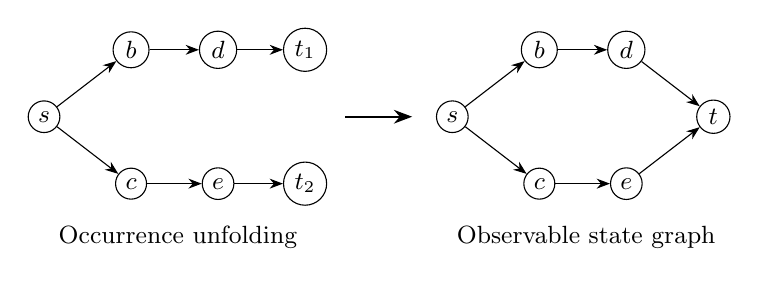
\begin{tikzpicture}[scale=.85,>=Stealth,
 every node/.style={font=\small},state/.style={circle,draw,inner sep=2pt}]
 \node[state] (a) at (0,0) {$s$};
 \node[state] (b) at (1.3,1) {$b$};
 \node[state] (d) at (2.6,1) {$d$};
 \node[state] (f1) at (3.9,1) {$t_1$};
 \node[state] (c) at (1.3,-1) {$c$};
 \node[state] (e) at (2.6,-1) {$e$};
 \node[state] (f2) at (3.9,-1) {$t_2$};
 \foreach \u/\v in {a/b,b/d,d/f1,a/c,c/e,e/f2}
     \draw[->] (\u)--(\v);
 \node at (2,-1.8) {Occurrence unfolding};
 \draw[->,thick] (4.5,0)--(5.5,0);
 \node[state] (aa) at (6.1,0) {$s$};
 \node[state] (bb) at (7.4,1) {$b$};
 \node[state] (dd) at (8.7,1) {$d$};
 \node[state] (ff) at (10,0) {$t$};
 \node[state] (cc) at (7.4,-1) {$c$};
 \node[state] (ee) at (8.7,-1) {$e$};
 \foreach \u/\v in {aa/bb,bb/dd,dd/ff,aa/cc,cc/ee,ee/ff}
     \draw[->] (\u)--(\v);
 \node at (8.1,-1.8) {Observable state graph};
\end{tikzpicture}
\caption{The case $k=2$, $L=3$. Identifying the final occurrences
creates a six-cycle. No independent events supply a square.}
\label{fig:cycle}
\end{figure}

These one-token rules can be read as replacements of typed unary
hyperedges at one immutable vertex. They are therefore instances
of the model in Theorem~\ref{thm:history}.
The example concerns a restricted family of rewrite systems; it
does not say that every state quotient has nonpositive curvature
or that every system with confluence fails to preserve geometry.

\section{Scope and reproduction}

There are three separate operations. Relabelling incidence positions
gives a symmetry quotient with inverse-automorphism weights.
Forgetting schedules gives linear-extension fibres and the extra
weight in \eqref{eq:scheduleweight}. Observing token states makes
further identifications, whose compatibility with the history median
is tested by Theorems~\ref{thm:observation} and~\ref{thm:matrix}.
Neither of the first two operations proves that the last preserves
geometry.

The known CAT(0) description supplies an exact finite geometry of
occurrences. A geometric assertion about observable states needs
control of the observation map. The repair problem in
Proposition~\ref{prop:repair} makes that requirement quantitative:
one must retain enough event information to separate the relevant
collisions. A continuum limit or a physical field equation would
require additional hypotheses and estimates, none of which is
implied by the torsor presentation.

The exact checker \path{check_history_states.py} compares wiring
restrictions with direct sequential execution, checks the incidence
weights, and exhaustively tests the observation criterion on all
partitions of ideal sets for naturally labelled posets through three
events. It also checks coordinate quotients, additive observations
through four events, repair sets, and the confluent families above.
The finite calculations supplement the proofs. Run
\texttt{make history-state-check} from the repository root.
All source inputs are TeX and bibliography files; the figure is
drawn directly in TeX.
The recorded run checks $4\,890$ partitions, of which $66$ inherit
the median, $706$ coordinate quotients and cube lifts, $3\,450$
additive observations and $2\,230$ repair sets. It constructs
$2\,742$ explicit failure witnesses and checks $16$ confluent
systems of the form \eqref{eq:chains}.

\bibliographystyle{abbrvurl}
\bibliography{history-states}
\end{document}
